%File: anonymous-submission-latex-2025.tex
\documentclass[letterpaper]{article} % DO NOT CHANGE THIS
\usepackage[]{aaai25}  % DO NOT CHANGE THIS
\usepackage{times}  % DO NOT CHANGE THIS
\usepackage{helvet}  % DO NOT CHANGE THIS
\usepackage{courier}  % DO NOT CHANGE THIS
\usepackage[hyphens]{url}  % DO NOT CHANGE THIS
\usepackage{graphicx} % DO NOT CHANGE THIS
\urlstyle{rm} % DO NOT CHANGE THIS
\def\UrlFont{\rm}  % DO NOT CHANGE THIS
\usepackage{natbib}  % DO NOT CHANGE THIS AND DO NOT ADD ANY OPTIONS TO IT
\usepackage{caption} % DO NOT CHANGE THIS AND DO NOT ADD ANY OPTIONS TO IT
\frenchspacing  % DO NOT CHANGE THIS
\setlength{\pdfpagewidth}{8.5in} % DO NOT CHANGE THIS
\setlength{\pdfpageheight}{11in} % DO NOT CHANGE THIS
\usepackage[outputdir=./temps]{minted}
%
% These are recommended to typeset algorithms but not required. See the subsubsection on algorithms. Remove them if you don't have algorithms in your paper.
\usepackage{algorithm}
\usepackage{algorithmic}

%
% These are are recommended to typeset listings but not required. See the subsubsection on listing. Remove this block if you don't have listings in your paper.
\usepackage{newfloat}
\usepackage{kotex}
\usepackage{listings}
\DeclareCaptionStyle{ruled}{labelfont=normalfont,labelsep=colon,strut=off} % DO NOT CHANGE THIS
\lstset{%
	basicstyle={\footnotesize\ttfamily},% footnotesize acceptable for monospace
	numbers=left,numberstyle=\footnotesize,xleftmargin=2em,% show line numbers, remove this entire line if you don't want the numbers.
	aboveskip=0pt,belowskip=0pt,%
	showstringspaces=false,tabsize=2,breaklines=true}
\floatstyle{ruled}
\newfloat{listing}{tb}{lst}{}
\floatname{listing}{Listing}
%
% Keep the \pdfinfo as shown here. There's no need
% for you to add the /Title and /Author tags.
\pdfinfo{
/TemplateVersion (2025.1)
}

% DISALLOWED PACKAGES
% \usepackage{authblk} -- This package is specifically forbidden
% \usepackage{balance} -- This package is specifically forbidden
% \usepackage{color (if used in text)
% \usepackage{CJK} -- This package is specifically forbidden
% \usepackage{float} -- This package is specifically forbidden
% \usepackage{flushend} -- This package is specifically forbidden
% \usepackage{fontenc} -- This package is specifically forbidden
% \usepackage{fullpage} -- This package is specifically forbidden
% \usepackage{geometry} -- This package is specifically forbidden
% \usepackage{grffile} -- This package is specifically forbidden
% \usepackage{hyperref} -- This package is specifically forbidden
% \usepackage{navigator} -- This package is specifically forbidden
% (or any other package that embeds links such as navigator or hyperref)
% \indentfirst} -- This package is specifically forbidden
% \layout} -- This package is specifically forbidden
% \multicol} -- This package is specifically forbidden
% \nameref} -- This package is specifically forbidden
% \usepackage{savetrees} -- This package is specifically forbidden
% \usepackage{setspace} -- This package is specifically forbidden
% \usepackage{stfloats} -- This package is specifically forbidden
% \usepackage{tabu} -- This package is specifically forbidden
% \usepackage{titlesec} -- This package is specifically forbidden
% \usepackage{tocbibind} -- This package is specifically forbidden
% \usepackage{ulem} -- This package is specifically forbidden
% \usepackage{wrapfig} -- This package is specifically forbidden
% DISALLOWED COMMANDS
\nocopyright
% \addtolength -- This command may not be used
% \balance -- This command may not be used
% \baselinestretch -- Your paper will not be published if you use this command
% \clearpage -- No page breaks of any kind may be used for the final version of your paper
% \columnsep -- This command may not be used
% \newpage -- No page breaks of any kind may be used for the final version of your paper
% \pagebreak -- No page breaks of any kind may be used for the final version of your paperr
% \pagestyle -- This command may not be used
% \tiny -- This is not an acceptable font size.
% \vspace{- -- No negative value may be used in proximity of a caption, figure, table, section, subsection, subsubsection, or reference
% \vskip{- -- No negative value may be used to alter spacing above or below a caption, figure, table, section, subsection, subsubsection, or reference

\setcounter{secnumdepth}{0} %May be changed to 1 or 2 if section numbers are desired.

% The file aaai25.sty is the style file for AAAI Press
% proceedings, working notes, and technical reports.
%

% Title

% Your title must be in mixed case, not sentence case.
% That means all verbs (including short verbs like be, is, using,and go),
% nouns, adverbs, adjectives should be capitalized, including both words in hyphenated terms, while
% articles, conjunctions, and prepositions are lower case unless they
% directly follow a colon or long dash
\title{발음 기반 한글 자연어 처리 Encoder \\
        Progress Report}
\author{
    % %Authors
    % % All authors must be in the same font size and format.
    % Written by AAAI Press Staff\textsuperscript{\rm 1}\thanks{With help from the AAAI Publications Committee.}\\
    % AAAI Style Contributions by Pater Patel Schneider,
    % Sunil Issar,\\
    % J. Scott Penberthy,
    % George Ferguson,
    % Hans Guesgen,
    % Francisco Cruz\equalcontrib,
    % Marc Pujol-Gonzalez\equalcontrib
    pronouncy
}
\affiliations{
    %Afiliations
    % \textsuperscript{\rm 1}Association for the Advancement of Artificial Intelligence\\
    % If you have multiple authors and multiple affiliations
    % use superscripts in text and roman font to identify them.
    % For example,

    % Sunil Issar\textsuperscript{\rm 2},
    % J. Scott Penberthy\textsuperscript{\rm 3},
    % George Ferguson\textsuperscript{\rm 4},
    % Hans Guesgen\textsuperscript{\rm 5}
    % Note that the comma should be placed after the superscript

    % 1101 Pennsylvania Ave, NW Suite 300\\
    % Washington, DC 20004 USA\\
    % % email address must be in roman text type, not monospace or sans serif
    % proceedings-questions@aaai.org
    김건형, 이준연, 구동한
%
% See more examples next
}

%Example, Single Author, ->> remove \iffalse,\fi and place them surrounding AAAI title to use it
\iffalse
\title{My Publication Title --- Single Author}
\author {
    Author Name
}
\affiliations{
    Affiliation\\
    Affiliation Line 2\\
    name@example.com
}
\fi

\iffalse
%Example, Multiple Authors, ->> remove \iffalse,\fi and place them surrounding AAAI title to use it
\title{My Publication Title --- Multiple Authors}
\author {
    % Authors
    First Author Name\textsuperscript{\rm 1},
    Second Author Name\textsuperscript{\rm 2},
    Third Author Name\textsuperscript{\rm 1}
}
\affiliations {
    % Affiliations
    \textsuperscript{\rm 1}Affiliation 1\\
    \textsuperscript{\rm 2}Affiliation 2\\
    firstAuthor@affiliation1.com, secondAuthor@affilation2.com, thirdAuthor@affiliation1.com
}
\fi


% REMOVE THIS: bibentry
% This is only needed to show inline citations in the guidelines document. You should not need it and can safely delete it.
\usepackage{bibentry}
% END REMOVE bibentry

\begin{document}

\maketitle

\begin{abstract}
한국어 학습자에게 있어 한글 발음과 실제 표기 간의 차이는 큰 장벽이 될 수 있다. 
특히 한국어는 음운 변화가 복잡하여 발음과 표기가 일치하지 않는 경우가 많다. 이러한 문제를 해결하기 위해, 본 프로젝트에서는 기존의 Text Encoder와 Phonetic Encoder를 결합한 FeatureFusion을 설계하고, 이를 통해 발음 정보를 포함한 한국어 처리를 가능하게 하는 시스템을 개발하고자 한다. 
이를 위해, 한국어 발음을 벡터화하여 유사 발음을 가진 단어들끼리 가까운 벡터 공간에 위치하도록 하는 Phonetic Encoder를 설계하였다. 
또한 발음대로 잘못 표기된 단어 데이터셋 구축을 위해 G2PK\cite{park2019g2pk}를 변형하여 올바르게 표기된 문장에 대해 발음 기반으로 잘못 표기된 단어를 생성하는 시스템을 개발하였다.
본 보고서는 중간 진행 상황을 공유하고, 향후 연구 방향을 제시하는 것을 목적으로 한다. 코드는 \url{https://github.com/edenkim9741/Natural-Language-Processing-Project.git}에서 확인할 수 있다.
\end{abstract}

% Uncomment the following to link to your code, datasets, an extended version or similar.
%
% \begin{links}
%     \link{Code}{https://aaai.org/example/code}
%     \link{Datasets}{https://aaai.org/example/datasets}
%     \link{Extended version}{https://aaai.org/example/extended-version}
% \end{links}

\section{Introduction}
한국어는 발음과 표기가 일치하지 않는 경우가 많아, 한국어 학습자에게 있어 발음과 표기 간의 차이는 큰 장벽이 될 수 있다.
특히 한국어는 음운 변화가 복잡하여 발음과 표기가 그 주변 단어나 문맥에 따라 달라지는 경우가 많다. 예를 들어, `밟다'라는 단어는 `밥다'로 발음되지만, `밟은'이라는 단어는 `발븐'으로 발음된다. 이러한 문제를 해결하기 위해, 본 프로젝트에서는 TTS(Text-to-Speech)를 활용하여 발음 정보를 벡터화하고, 이를 통해 발음 기반의 단어 검색 시스템을 개발하고자 한다.
본 프로젝트의 기여는 다음과 같다.
\begin{itemize}
    \item 한국어에서 발음 기반의 모델의 필요성을 제기하고, 이를 해결하기 위한 Phonetic Encoder 설계
    \item 발음대로 잘못 표기된 단어 데이터셋 구축을 위한 G2PK 변형
    \item BertEncoder와 PhoneticEncoder를 결합한 FeatureFusion 설계 및 검증
\end{itemize}

\section{Related Works}
\subsection{G2PK}
G2PK(graphemes to phonemes for korean)에서는 한국어 문장을 입력받아 해당 문장의 발음을 추출하는 패키지이다.
Appendix G2PK Rule\ref{sec:g2pk_rule}에서 G2PK의 변형 규칙을 확인할 수 있다.
하지만 기존의 G2PK는 대부분 음운 규칙만을 따라 문장을 변형하기 때문에 한국어 학습자가 발음대로 잘못 표기한 단어를 생성하기에는 한계가 있다.
예를 들어, `있습니다'라는 단어는 G2PK에 의해 `읻씀니다'로 변형되지만, 한국어 학습자가 발음대로 잘못 표기할 수 있는 단어는 `잇습니다', `잇씁니다', `잇슴니다' 등 다양한 형태가 존재한다.

\subsection{Text Encoder}
소리나는대로 표기된 단어일지라도 기존 단어와 유사한 Token을 가질 수 있다. 
특히 소리나는대로 표기되었더라도 기존 단어와 형태가 변하지 않는 경우에는 Text Encoder로 처리되었을 때 기존 단어와 동일한 Token과 Embedding Vector를 가진다. 
예를 들어, `사과'라는 단어는 소리나는대로 표기하더라도 `사과'이므로 동일한 Token과 Embedding Vector를 가진다.

본 프로젝트에서 활용한 BertEncoder는 문장의 맥락적인 정보를 파악할 수 있기 때문에 주변의 단어를 통해서 발음대로 표기된 단어의 의미를 유추할 수 있다.

\subsection{Phonetic Encoder}
Phonetic Encoder는 텍스트로부터 생성된 음성의 발음 정보를 추출하여 고정된 벡터로 변환해주는 모듈이다.
기존의 Text Encoder는 정확한 철자 입력을 전제로 하기 때문에, 발음대로 잘못 표기된 단어와 문장을 Encoding 했을 때 정확한 문장을 Embedding한 Vector와 차이가 존재한다.

이러한 차이를 완화시키기 위해 본 프로젝트에서는 Phonetic Encoder를 사용하였다. 입력 텍스트를 TTS(Text-to Speech)를 통해 음성으로 변환하고, 해당 음성 데이터를 벡터화하여 발음 기반 유사도 비교가 가능하도록 한다. 이렇게 추출된 벡터는 유사 발음을 가지는 단어들끼리 가까운 벡터 공간에 위치하게 되어, 철자가 다르더라도 발음이 유사한 단어를 효과적으로 매칭할 수 있게 된다. 따라서 Phonetic Encoder는 오타 교정, 발음 기반의 검색, 외국어 학습 지원 등 다양한 음성 기반 응용에 핵심적인 역할을 할 수 있다.

\section{Dataset}
\begin{figure*}[ht]
    \centering
    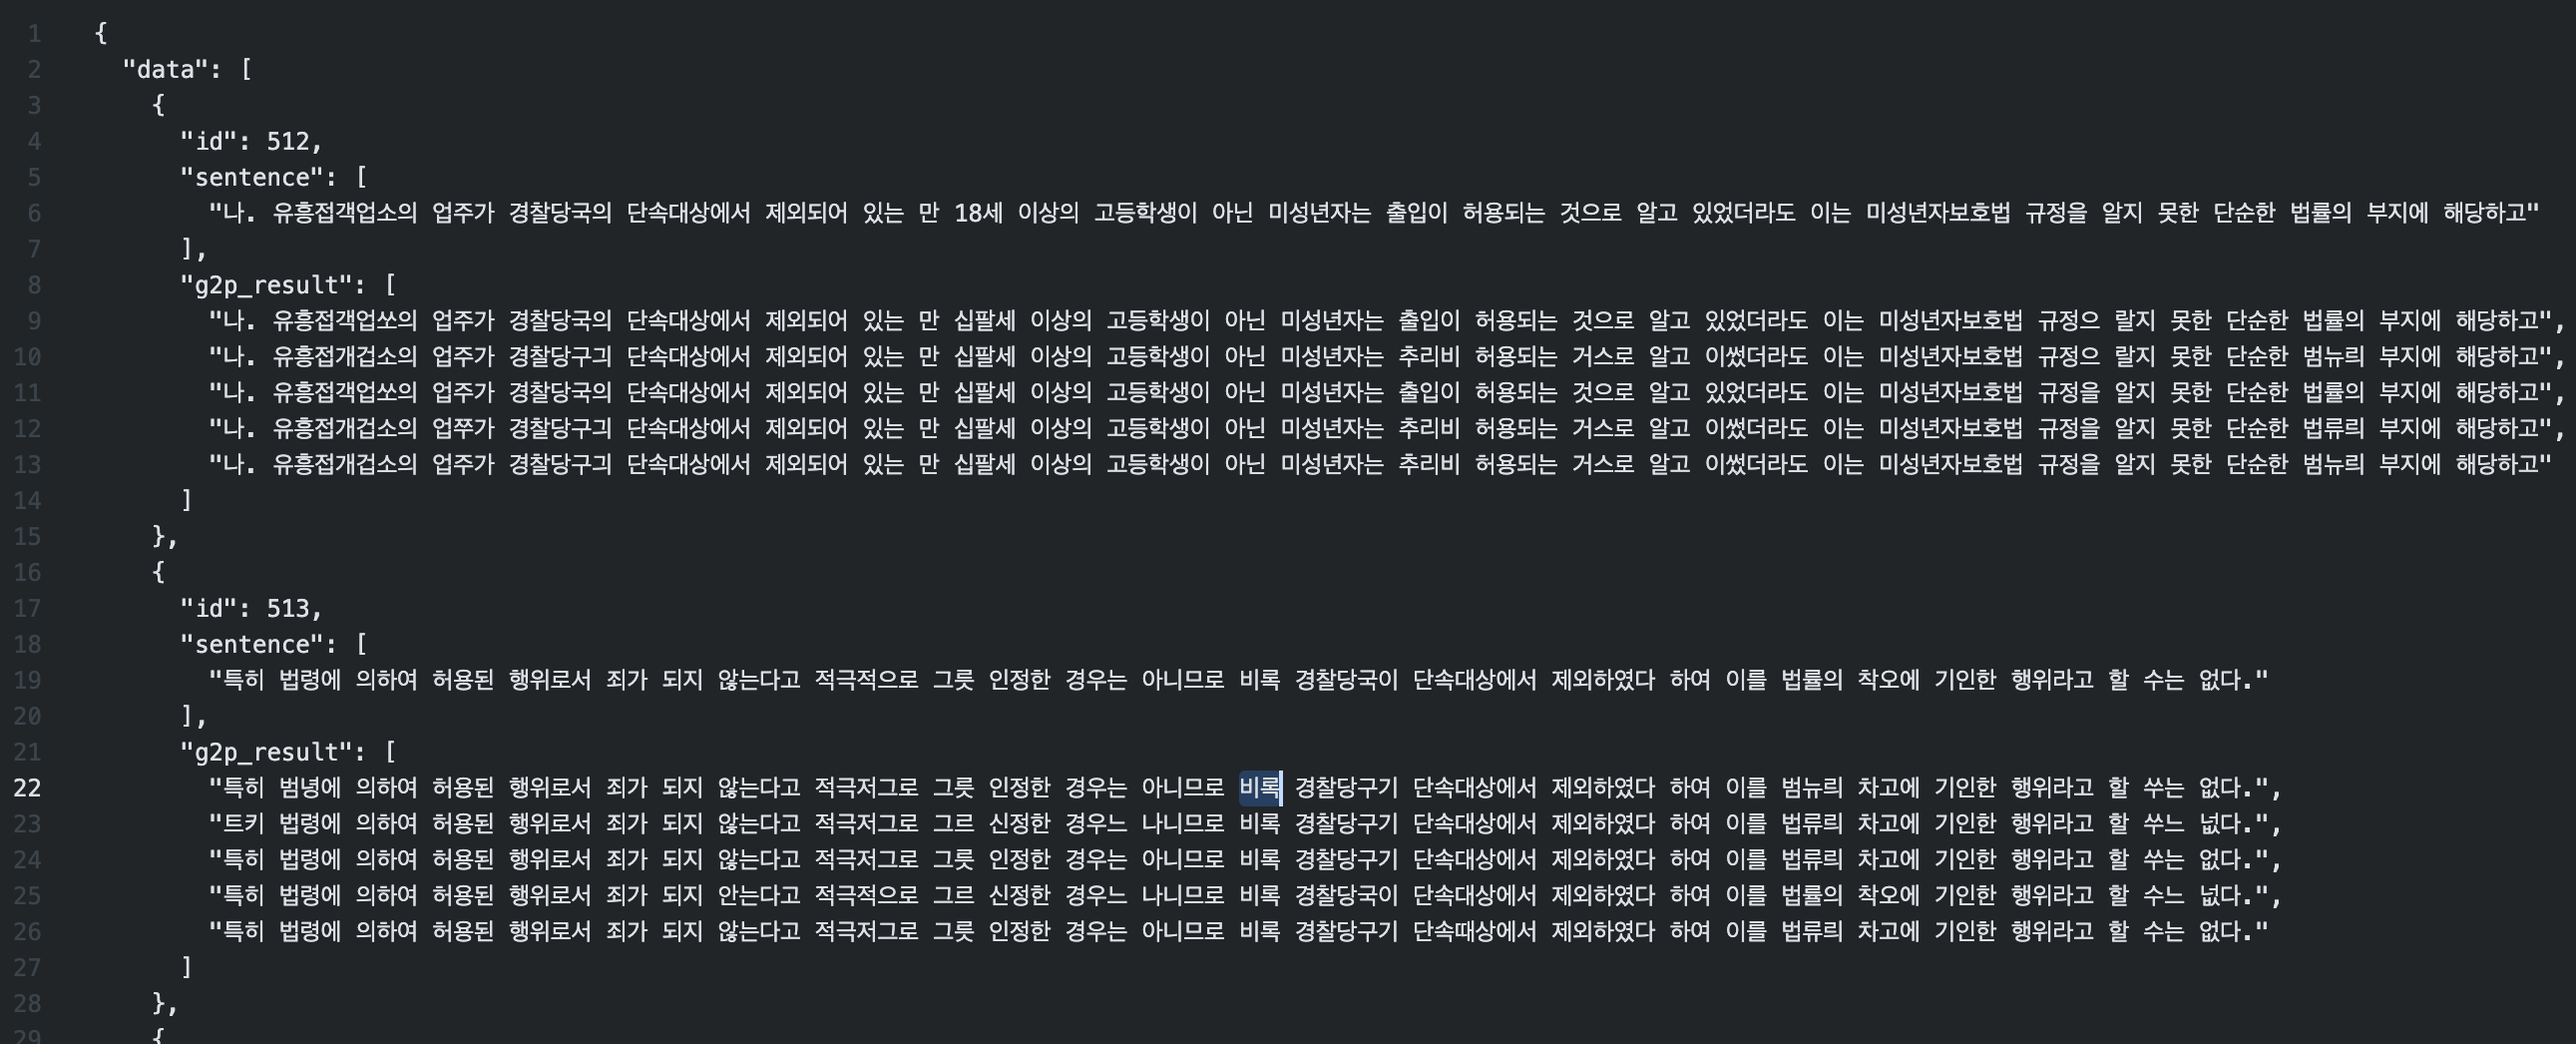
\includegraphics[width=0.8\textwidth]{figures/text_dataset_example.png}
    \caption{Text Dataset Example}
    \label{fig:text_dataset_example}
\end{figure*}
\subsection{Text Dataset}
Text Dataset은 올바른 한국어 문장을 통해 생성되었다. Dataset은 json 파일 형식으로 문장의 번호와 올바른 문장(1개), 한국어 학습자가 발음대로 잘못 표기할 수 있는 문장 최대 5개로 이루어져있다. 해당 오류들은 Modifed G2PK를 통해 생성되었으며, 각 오류들은 G2PK의 문장 변형 과정에서 랜덤하게 선택된다. 추후에는 해당 문장이 어떤 오류를 포함하고 있는지에 대한 정보도 추가할 예정이다. Figure \ref{fig:text_dataset_example}은 Text Dataset의 예시를 보여준다.



\subsection{Phonetic Dataset}
Phonetic Dataset은 Text Dataset의 문장을 TTS(Text-to-Speech)를 통해 음성으로 변환한 wav 파일과 해당 wav 파일을 Wav2Vec2를 통해 벡터화한 결과로 구성된다.
gTTS의 제한으로 인해 현재 약 1600개의 문장에 대한 wav 파일만 생성되었으며, 추후에 다른 TTS 모델을 활용하여 나머지 문장에 대한 wav 파일을 생성할 예정이다.
또한 TTS의 음색을 달리하여 다양한 발음 정보를 포함한 wav 파일을 생성해보고 해당 데이터를 활용했을 때에 대한 실험도 진행할 예정이다.

\section{Methods}

\begin{figure*}[ht]
    \centering
    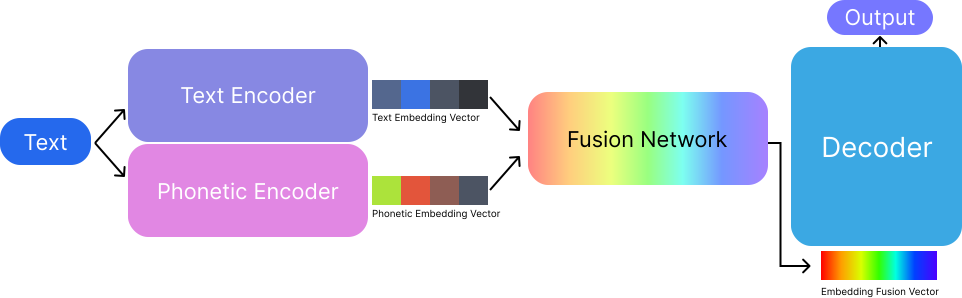
\includegraphics[width=0.8\textwidth]{figures/phonetic_fusion_embedding.pdf}
    \caption{Phonetic Fusion Embedding Architecture}
    \label{fig:phonetic_encoder}
\end{figure*}

\subsection{Modified G2PK}
기존 G2PK는 음운 규칙에 따라 문장을 변형하는 방식으로, 한국어 학습자가 발음대로 잘못 표기한 단어를 생성하기에는 한계가 있다.
따라서 본 프로젝트에서는 아래와 같은 규칙을 추가하여 한국어 학습자가 발음대로 잘못 표기할 수 있는 단어들을 생성하는 시스템을 개발하였다.
\begin{itemize}
  \item 한국어 학습자가 제대로 표기하는 방법을 알고 있는 경우를 고려하여 제대로 표기하는 경우도 모든 규칙에 대해 추가한다.
  \begin{itemize}
    \item 있습니다[있습니다, 읻씀니다, 잇슴니다, ...]
  \end{itemize}
  \item 한국어 학습자가 받침을 표기할 때 'ㅅ, ㅆ, ㅈ, ㅊ, ㅌ'을 [ㅅ, ㅆ]으로 표기하는 경우가 있다.
  \begin{itemize}
    \item 썼다[썻따]
    \item 쫓다[쫏따]
    \item 쫓기다[쫏끼다]
  \end{itemize}
  \item 용언의 어간 말음 `ㄺ'은 `ㄱ' 앞에서 [ㄹ]로 발음하지만, 한국어 학습자는 `ㄱ'으로 발음하는 경우가 있다.
  \begin{itemize}
    \item 맑게[말께, 막께]
    \item 묽고[물꼬, 묵꼬]
    \item 읽거나[일꺼나, 익꺼나]
  \end{itemize}
\end{itemize}


\subsection{BertEncoder}
BertEncoder는 입력된 문장을 BertTokenizer를 통해 Tokenize하고, 이를 BertModel에 입력하여 문장의 Embedding Vector를 생성한다.
BertTokenizer와 BertModel은 HuggingFace에서 제공하는 pre-trained 모델을 사용했다. 추후에 다른 모델들을 활용하여 성능을 비교하는 실험도 추가할 예정이다.

BertEncoder에서 feature Vector를 추출하기 위해서 extract\_features 함수를 사용하였다. 이 함수는 입력된 문장을 BertTokenizer를 통해 Tokenize하고, 이를 BertModel에 입력하여 문장의 Embedding Vector를 생성한다.
이렇게 생성된 Text Vector $\mathbf{v}_t$는 [T, 768]의 크기를 가진다.
Embedding Vector를 생성하는 방식으로는 cls token, mean pooling, max pooling을 선택할 수 있도록 하였고, 각각의 방식에 따른 $\mathbf{v}_t$들의 정답과의 유사도를 비교하는 실험을 진행했다.




\subsection{PhoneticEncoder}
PhoneticEncoder는 입력된 문장을 TTS(Text-to-Speech)를 통해 음성으로 변환하고, 이를 Wav2Vec2를 통해 벡터화한 후에 GRU 기반의 RNN을 통해 시퀀스 벡터를 처리하여 발음 정보를 포함한 고정된 크기의 벡터를 생성한다.
\subsubsection{TTS}
입력으로 들어온 Text를 TTS(Text-to-Speech)로 wav 파일로 변환하기 위해 gTTS를 사용하고 있다. gTTS도 API의 제한이 존재하기 때문에 다른 Local에서 실행가능한 TTS를 활용하여 데이터셋을 모두 생성할 예정이다.

\subsubsection{Wav2Vec2}
Wav2Vec2 기반의 발음 임베딩 생성을 위해, 먼저 torchaudio를 활용하여 wav 파일을 로드하였고, 샘플링 레이트를  16kHz로 정규화하였다. 
이렇게 정규화된 waveform을 HuggingFace에서 제공하는 Wav2Vec2Processor에 입력하여(Wav2Vec2Model을 활용), 적절한 입력 format으로 변환한 뒤, Wav2Vec2Model의 출력에서 마지막 hidden state를 추출하였다. 
최종적으로 [T, 768] 크기의 시퀀스 벡터가 생성되며, 이는 이후 Phonetic Encoder로 전달된다.

\subsubsection{Phonetic Encoder}
Phonetic Encoder는 Wav2Vec2로부터 추출된 시퀀스 벡터를 입력으로 받아 GRU 기반의 RNN을 통해 시퀀스 벡터를 처리한다.
최종적으로 처리된 벡터는 Phonetic Vector $\mathbf{v}_p$로 표현되며, 이는 발음 정보를 포함한 고정된 크기의 벡터이다. 이 벡터는 발음 기반의 유사도 비교를 위해 사용된다.
추후에는 GRU 기반의 RNN 외에도 Transformer 기반의 모델을 활용하여 성능을 비교하는 실험도 진행할 예정이다.

\subsection{FeatureFusion}
FeatureFusion은 BertEncoder와 PhoneticEncoder의 출력 벡터를 결합하여 최종 임베딩 벡터를 생성하는 모듈이다.
이를 위해 BertEncoder와 PhoneticEncoder의 출력 벡터를 결합한 후 pytorch에서 제공하는 간단한 FC(Fully Connected) Layer를 사용하여 projection하였다. 이렇게 최종적으로 추출된 Embedding Vector $\mathbf{v}_f$는 발음과 문맥 정보를 모두 포함한 벡터로, 발음 기반의 유사도 비교를 가능하게 한다.

이는 다음과 같은 수식으로 표현할 수 있다.
\begin{equation}
    \mathbf{v}_f = FC (\mathbf{v}_t \oplus \mathbf{v}_p)
\end{equation}

\subsection{Decoder}
Encoder에서의 Feature가 얼마나 효과적으로 추출되었는지를 평가하기 위해, Decoder를 도입하여 여러 Downstream Task에 대한 성능을 평가할 예정이다.
현재 계획중인 Downstream Task는 다음과 같다.
\begin{itemize}
    \item 번역
    \item 오류 교정 (정답 문장 Reconstuction)
\end{itemize}

\section{Experiments}
\subsection{Experimental Setup}
본 프로젝트에서는 인공지능혁신융합대학사업단의 장비대여 사업을 통해 NVIDIA A100 GPU(20gb)를 사용하여 진행하였다.

\subsection{Text Encoder와 Phonetic Encoder의 유사도 비교}
실제로 Phonetic Feature를 도입하는 것이 효과가 있는지에 대해 확인하기 위해 정답 문장에서 각각 Text Encoder, Phonetic Encoder로 추출한 벡터 $\mathbf{v}_{t,T}, \mathbf{v}_{p,T}$에 대해서 $i$번째 오류 문장을 각각의 Encoder로 추출한 벡터 $\mathbf{v}_{t,i}, \mathbf{v}_{p,i}$의 유사도의 평균을 비교하였다.
\begin{equation}
    avg\_similarity_{t} = \frac{1}{N} \sum_{i=1}^{N} \frac{\mathbf{v}_{t,T} \cdot \mathbf{v}_{t,i}}{||\mathbf{v}_{t,T}|| \cdot ||\mathbf{v}_{t,i}||}
\end{equation}
\begin{equation}
    avg\_similarity_{p} = \frac{1}{N} \sum_{i=1}^{N} \frac{\mathbf{v}_{p,T} \cdot \mathbf{v}_{p,i}}{||\mathbf{v}_{p,T}|| \cdot ||\mathbf{v}_{p,i}||}
\end{equation}
\begin{table}[ht]
    \centering
    \begin{tabular}{lcc}
    Pooling & \multicolumn{1}{l}{Text Encoder} & \multicolumn{1}{l}{Phonetic Encoder} \\ \hline
    CLS     & 0.9597                           &                                      \\
    Mean    & 0.9069                           & 0.9934                               \\
    Max     & 0.9621                           &                                     
    \end{tabular}
    \caption{Text Encoder와 Phonetic Encoder의 유사도 비교 결과}
    \label{tab:encoder_comparison}
\end{table}

비교 결과 Table \ref{tab:encoder_comparison}과 같이 Phonetic Encoder의 Feature Vector가 Text Encoder의 Feature Vector보다 평균 유사도가 높게 나타났다. 이 결과는 Phonetic Encoder가 Modified G2PK로 생성된 발음대로 잘못 표기된 단어들에 대해서 더 강건함을 보여준다.

\begin{figure}[ht]
    \centering
    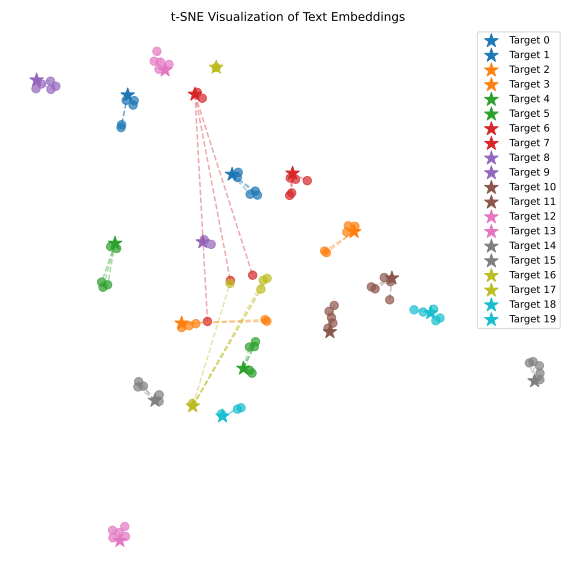
\includegraphics[width=0.45\textwidth]{figures/tsne_text_embeddings.pdf}
    \caption{Text Encoder의 Embedding Space}
    \label{fig:tsne_text_encoder}
\end{figure}

\begin{figure}[ht]
    \centering
    \includegraphics[width=0.45\textwidth]{figures/tsne_phonetic_embeddings.pdf}
    \caption{Phonetic Encoder의 Embedding Space}
    \label{fig:tsne_phonetic_encoder}
\end{figure}

\subsection{Text Encoder와 Phonetic Encoder의 Embedding Space 비교}
단순 유사도를 비교하는 것은 negetive pair에 대한 유사도를 반영하고 있지 않기 때문에 t-SNE를 활용하여 서로 다른 문장 간의 거리를 유지하면서 Embedding Space를 효과적으로 생성하고 있는지 확인하였다. 
Figure \ref{fig:tsne_text_encoder}와 Figure \ref{fig:tsne_phonetic_encoder}는 각각 20개의 문장에 대해 Text Encoder와 Phonetic Encoder로 추출한 Embedding Space를 시각화한 결과이다.

결과를 살펴보면 

\section{Future Plans}
\subsection{Text Dataset 개선 및 Phonetic Dataset 확장}
현재 Text Dataset은 랜덤하게 5개의 오류 문장을 생성하는 방식으로 구성되어 있지만 생성된 문장이 어떤 오류를 포함하고 있는지에 대한 정보는 없다. 
json 파일에 어떠한 오류로부터 생성된 문장인지에 대한 정보를 추가하여, Downstream Task에서 어떤 오류에 대한 성능이 좋고 나쁜지에 대한 분석을 할 수 있도록 개선할 예정이다.

또한 Phonetic Dataset은 API의 제한으로 인해 현재 약 1600개의 문장에 대한 wav 파일만 생성되었으며, 나머지 문장에 대한 wav 파일을 생성할 예정이다.

\subsection{다양한 Text Encoder 적용}
현재 구현한 BertEncoder 외에 HuggingFace에서 제공하는 다양한 Text Encoder, 특히 한국어에 특화된 Encoder를 활용하여 성능을 비교할 예정이다. 
예를 들어, KoBERT, KoGPT 등의 모델이 발음 오류에 대한 강건성을 가지는지에 대해 집중적으로 실험할 예정이다.

\subsection{Transformer 기반 Phonetic Encoder 적용}
현재 GRU 기반의 Encoder도 Embedding Space를 확인했을 때 시각적으로는 좋은 성능을 확인할 수 있었지만, Downstream Task에는 적합하지 않은 Vecotor일 가능성이 있다. 
따라서 Transformer 기반의 Encoder를 활용하여 Phonetic Encoder를 개선하고 Downstream Task에 대해서 어떤 변화가 있는지에 대해 실험할 예정이다.

\subsection{Fusion Feature를 이용한 Downstream Task}
현재 FeatureFusion은 구현은 되어 있지만 학습은 되어 있지 않은 상태이다. (Phonetic Dataset의 부족으로 인해) 추후에 Phonetic Dataset을 확장하고, BertEncoder와 PhoneticEncoder를 결합한 FeatureFusion을 학습시킬 예정이다.

FeatureFusion에서 추출한 Embedding Vector $\mathbf{v}_f$를 활용하여 아래 Downstream Task에 대한 성능을 평가할 예정이다.
\begin{itemize}
    \item 번역: 발음대로 잘못 표기된 문장을 입력으로 받아 올바르게 번역하는 Task
    \item 오류 교정: 한국어 학습자가 발음대로 잘못 표기한 단어를 입력으로 받아 해당 문장을 올바르게 재구성하는 모델을 학습할 예정이다.
\end{itemize}


\clearpage
\section{Appendix}
\subsection{G2PK Rule} \label{sec:g2pk_rule}
G2PK는 다음과 같은 규칙으로 입력 문장을 발음대로 재구성한다.

\begin{minted}[breaklines, fontsize=\scriptsize]{markdown}
5.1
5항. 다만 1. 용언의 활용형에 나타나는 '져, 쪄, 쳐'는 [저, 쩌, 처]로 발음한다.
-> 가져[가저], 쪄[쩌], 다쳐[다처]

5.2
5항. 다만 2. '예, 례' 이외의 'ㅖ'는 [ㅔ]로도 발음한다.
-> 계집[계집/게집], 계시다[계시다/게시다]
-> 시계[시계/시게](時計), 연계[연계/연게](連繫)
-> 몌별[몌별/메별](袂別), 개폐[개폐/개페](開閉)
-> 혜택[혜택/헤택](惠澤), 지혜[지혜/지헤](智慧)
# 실제로 언중은 예, 녜, 셰, 쎼 이외의 'ㅖ'는 [ㅔ]로 발음한다. by kyubyong

5.3
5항. 다만 3. 자음을 첫소리로 가지고 있는 음절의 'ㅢ'는 [ㅣ]로 발음한다.
-> 늴리리[닐리리], 닁큼[닝큼], 무늬[무니], 띄어쓰기[띠어쓰기], 씌어[씨어]
-> 틔어[티어], 희어[히어], 희떱다[히떱따], 희망[히망], 유희[유히]

5.4.1
다만 4. 단어의 첫음절 이외의 '의'는 [ㅣ]로 발음함도 허용한다.
-> 주의[주의/주이], 협의[혀븨/혀비]
# 실제로 언중은 높은 확률로 단어의 첫음절 이외의 '의'는 [ㅣ]로 발음한다.

5.4.2
다만 4. 조사 '의'는 [ㅔ]로 발음함도 허용한다.
-> 우리의[우리의/우리에], 강의의[강의의/강이에]
# 실제로 언중은 높은 확률로 조사 '의'는 [ㅔ]로 발음한다.

9
제9항 받침 'ㄲ, ㅋ', 'ㅅ, ㅆ, ㅈ, ㅊ, ㅌ', 'ㅍ'은 어말 또는 자음 앞에서 각각 대표음 [ㄱ, ㄷ, ㅂ]으로 발음한다.
-> 닦다[닥따], 키읔[키윽], 키읔과[키윽꽈], 옷[옫]
-> 웃다[욷따], 있다[읻따], 젖[젇], 빚다[빋따]
-> 꽃[꼳], 쫓다[쫃따], 솥[솓], 뱉다[밷따]
-> 앞[압], 덮다[덥따]

10
제10항 겹받침 'ㄳ', 'ㄵ', 'ㄼ, ㄽ, ㄾ', 'ㅄ'은 어말 또는 자음 앞에서 각각 [ㄱ, ㄴ, ㄹ, ㅂ]으로 발음한다.
-> 넋[넉], 넋과[넉꽈], 앉다[안따], 여덟[여덜]
-> 넓다[널따], 외곬[외골], 핥다[할따], 값[갑]
-> 없다[업:따]

10.1
다만, '밟-'은 자음 앞에서 [밥]으로 발음하고, '넓-'은 다음과 같은 경우에 [넙]으로 발음한다.
-> 1) 밟다[밥따], 밟소[밥쏘], 밟지[밥찌], 밟는[밤:는], 밟게[밥께], 밟고[밥꼬]
-> 2) 넓죽하다[넙쭈카다], 넓둥글다[넙뚱글다]

11
제11항 겹받침 'ㄺ, ㄻ, ㄿ'은 어말 또는 자음 앞에서 각각 [ㄱ, ㅁ, ㅂ]으로 발음한다.
-> 닭[닥], 흙과[흑꽈], 맑다[막따], 늙지[늑찌]
-> 삶[삼], 젊다[점따], 읊고[읍꼬], 읊다[읍따]

11.1
다만, 용언의 어간 말음 'ㄺ'은 'ㄱ' 앞에서 [ㄹ]로 발음한다.
-> 맑게[말께], 묽고[물꼬], 읽거나[일꺼나]

12
제12항 받침 'ㅎ'의 발음은 다음과 같다.
1. 'ㅎ(ㄶ, ㅀ)' 뒤에 'ㄱ, ㄷ, ㅈ'이 결합되는 경우에는, 뒤 음절 첫소리와 합쳐서 [ㅋ, ㅌ, ㅊ]으로 발음한다.
-> 놓고[노코], 좋던[조턴], 쌓지[싸치], 많고[만코]
-> 않던[안턴], 닳지[달치]
[붙임 1] 받침 'ㄱ(ㄺ), ㄷ, ㅂ(ㄼ), ㅈ(ㄵ)'이 뒤 음절 첫소리 'ㅎ'과 결합되는 경우에도, 역시 두 소리를 합쳐서 [ㅋ, ㅌ, ㅍ, ㅊ]으로 발음한다.
-> 각하[가카], 먹히다[머키다], 밟히다[발피다], 맏형[마텽]
-> 좁히다[조피다], 넓히다[널피다], 꽂히다[꼬치다], 앉히다[안치다]
[붙임 2] 규정에 따라 'ㄷ'으로 발음되는 'ㅅ, ㅈ, ㅊ, ㅌ'의 경우에는 이에 준한다.
-> 옷 한 벌[오 탄 벌], 낮 한때[나 탄때], 꽃 한 송이[꼬 탄 송이]
-> 숱하다[수타다]
2. 'ㅎ(ㄶ, ㅀ)' 뒤에 'ㅅ'이 결합되는 경우에는, 'ㅅ'을 [ㅆ]으로 발음한다.
-> 닿소[다쏘], 많소[만쏘], 싫소[실쏘]
3. 'ㅎ' 뒤에 'ㄴ'이 결합되는 경우에는, [ㄴ]으로 발음한다.
-> 놓는[논는], 쌓네[싼네]
[붙임] 'ㄶ, ㅀ' 뒤에 'ㄴ'이 결합되는 경우에는, 'ㅎ'을 발음하지 않는다.
-> 않네[안네], 않는[안는], 뚫네[뚤레], 뚫는[뚤른]
- '뚫네[뚤네→뚤레], 뚫는[뚤는→뚤른]'에 대해서는 제20항 참조.

12.4
4. 'ㅎ(ㄶ, ㅀ)' 뒤에 모음으로 시작된 어미나 접미사가 결합되는 경우에는, 'ㅎ'을 발음하지 않는다.
-> 낳은[나은], 놓아[노아], 쌓이다[싸이다], 많아[마나]
-> 않은[아는], 닳아[다라], 싫어도[시러도]

13
제13항 홑받침이나 쌍받침이 모음으로 시작된 조사나 어미, 접미사와 결합되는 경우에는, 제 음가대로 뒤 음절 첫소리로 옮겨 발음한다.
-> 깎아[까까], 옷이[오시], 있어[이써], 낮이[나지]
-> 꽂아[꼬자], 꽃을[꼬츨], 쫓아[쪼차], 밭에[바테]
-> 앞으로[아프로], 덮이다[더피다]

14
제14항 겹받침이 모음으로 시작된 조사나 어미, 접미사와 결합되는 경우에는, 뒤엣것만을 뒤 음절 첫소리로 옮겨 발음한다. (이 경우, 'ㅅ'은 된소리로 발음함.)
-> 넋이[넉씨], 앉아[안자], 닭을[달글], 젊어[절머]
-> 곬이[골씨], 핥아[할타], 읊어[을퍼], 값을[갑쓸]
-> 없어[업써]

15
제15항 받침 뒤에 모음 'ㅏ, ㅓ, ㅗ, ㅜ, ㅟ'들로 시작되는 실질 형태소가 연결되는 경우에는, 대표음으로 바꾸어서 뒤 음절 첫소리로 옮겨 발음한다.
-> 밭 아래[바 다래] 		늪 앞[느 밥] 		젖어미[저더미] 		맛없다[마덥다]
-> 겉옷[거돋] 		헛웃음[허두슴] 		꽃 위[꼬 뒤]
다만, '맛있다, 멋있다'는 [마싣따], [머싣따]로도 발음할 수 있다.
[붙임] 겹받침의 경우에는 그 중 하나만을 옮겨 발음한다.
-> 넋 없다[너 겁따] 		닭 앞에[다 가페] 		값어치[가 버치] 		값있는[가빈는]

16
제16항 한글 자모의 이름은 그 받침소리를 연음하되, 'ㄷ, ㅈ, ㅊ, ㅋ, ㅌ, ㅍ, ㅎ'의 경우에는 특별히 다음과 같이 발음한다.
-> 디귿이[디그시], 디귿을[디그슬], 디귿에[디그세]
-> 지읒이[지으시], 지읒을[지으슬], 지읒에[지으세]
-> 치읓이[치으시], 치읓을[치으슬], 치읓에[치으세]
-> 키읔이[키으기], 키읔을[키으글], 키읔에[키으게]
-> 티읕이[티으시], 티읕을[티으슬], 티읕에[티으세]
-> 피읖이[피으비], 피읖을[피으블], 피읖에[피으베]
-> 히읗이[히으시], 히읗을[히으슬], 히읗에[히으세]

17
제17항 받침 'ㄷ, ㅌ(ㄾ)'이 조사나 접미사의 모음 'ㅣ'와 결합되는 경우에는, [ㅈ, ㅊ]으로 바꾸어서 뒤 음절 첫소리로 옮겨 발음한다.
-> 곧이듣다[고지듣따], 굳이[구지], 미닫이[미다지]
-> 땀받이[땀바지], 밭이[바치], 벼훑이[벼훌치]
[붙임] 'ㄷ' 뒤에 접미사 '히'가 결합되어 '티'를 이루는 것은 [치]로 발음한다.
-> 굳히다[구치다], 닫히다[다치다], 묻히다[무치다]

18
제18항 받침 'ㄱ(ㄲ, ㅋ, ㄳ, ㄺ), ㄷ(ㅅ, ㅆ, ㅈ, ㅊ, ㅌ, ㅎ), ㅂ(ㅍ, ㄼ, ㄿ, ㅄ)'은 'ㄴ, ㅁ' 앞에서 [ㅇ, ㄴ, ㅁ]으로 발음한다.
-> 먹는[멍는], 국물[궁물], 깎는[깡는], 키읔만[키응만]
-> 몫몫이[몽목씨], 긁는[긍는], 흙만[흥만], 닫는[단는]
-> 짓는[진:는], 옷맵시[온맵시], 있는[인는], 맞는[만는]
-> 젖멍울[전멍울], 쫓는[쫀는], 꽃망울[꼰망울], 붙는[분는]
-> 놓는[논는], 잡는[잠는], 밥물[밤물], 앞마당[암마당]
-> 밟는[밤:는], 읊는[음는], 없는[엄:는], 값매다[감매다]
[붙임] 두 단어를 이어서 한 마디로 발음하는 경우에도 이와 같다.
-> 책 넣는다[챙 넌는다], 흙 말리다[흥 말리다], 옷 맞추다[온 마추다]
-> 밥 먹는다[밤 멍는다], 값 매기다[감 매기다]

19
제19항 받침 'ㅁ, ㅇ' 뒤에 연결되는 'ㄹ'은 [ㄴ]으로 발음한다.
-> 담력[담:녁], 침략[침냑], 강릉[강능], 항로[항:노], 대통령[대:통녕]
[붙임] 받침 'ㄱ, ㅂ' 뒤에 연결되는 'ㄹ'도 [ㄴ]으로 발음한다.
-> 막론[막논→망논], 백리[백니→뱅니], 협력[협녁→혐녁], 십리[십니→심니]

20
제20항 'ㄴ'은 'ㄹ'의 앞이나 뒤에서 [ㄹ]로 발음한다.
-> 1) 난로[날:로], 신라[실라], 천리[철리], 광한루[광:할루], 대관령[대:괄령]
-> 2) 칼날[칼랄], 물난리[물랄리], 줄넘기[줄럼끼], 할는지[할른지]
[붙임] 첫소리 'ㄴ'이 'ㅀ, ㄾ' 뒤에 연결되는 경우에도 이에 준한다.
-> 닳는[달른], 뚫는[뚤른], 핥네[할레]
다만, 다음과 같은 단어들은 'ㄹ'을 [ㄴ]으로 발음한다.
-> 의견란[의견난], 임진란[임진난], 생산량[생산냥]
-> 결단력[결딴녁], 공권력[공꿘녁], 동원령[동:원녕]
-> 상견례[상견녜], 횡단로[횡단노], 이원론[이원논]
-> 입원료[이붠뇨], 구근류[구근뉴]

21
제21항 위에서 지적한 이외의 자음 동화는 인정하지 않는다.
-> 감기[감기], 옷감[옫깜], 있고[읻꼬]
-> 꽃길[꼳낄],	젖먹이[전머기], 문법[문뻡]
-> 꽃밭[꼳빧]

22
제22항 다음과 같은 용언의 어미는 [어]로 발음함을 원칙으로 하되, [여]로 발음함도 허용한다.
-> 피어[피어/피여] 		되어[되어/되여]
[붙임] '이오, 아니오'도 이에 준하여 [이요, 아니요]로 발음함을 허용한다.

23
제23항 받침 'ㄱ(ㄲ, ㅋ, ㄳ, ㄺ), ㄷ(ㅅ, ㅆ, ㅈ, ㅊ, ㅌ), ㅂ(ㅍ, ㄼ, ㄿ, ㅄ)' 뒤에 연결되는 'ㄱ, ㄷ, ㅂ, ㅅ, ㅈ'은 된소리로 발음한다.
-> 국밥[국빱], 깎다[깍따], 넑받이[넉빠지], 삯돈[삭똔]
-> 닭장[닥짱], 칡범[칙뻠], 뻗대다[뻗때다], 옷고름[옫꼬름]
-> 있던[읻떤], 꽂고[꼳꼬], 꽃다발[꼳따발], 낯설다[낟썰다]
-> 밭갈이[받까리], 솥전[솓쩐], 곱돌[곱똘], 덮개[덥깨]
-> 옆집[엽찝], 넓죽하다[넙쭈카다], 읊조리다[읍쪼리다], 값지다[갑찌다]

24
제24항 어간 받침 'ㄴ(ㄵ), ㅁ(ㄻ)' 뒤에 결합되는 어미의 첫소리 'ㄱ, ㄷ, ㅅ, ㅈ'은 된소리로 발음한다.
-> 신고[신꼬], 껴안다[껴안따], 앉고[안꼬], 얹다[언따]
-> 삼고[삼꼬], 더듬지[더듬찌], 닮고[담꼬], 젊지[점찌]
다만, 피동, 사동의 접미사 '-기-'는 된소리로 발음하지 않는다.
-> 안기다[안기다], 감기다[감기다], 굶기다[굼기다], 옮기다[옴기다]

25
제25항 어간 받침 'ㄼ, ㄾ' 뒤에 결합되는 어미의 첫소리 'ㄱ, ㄷ, ㅅ, ㅈ'은 된소리로 발음한다.
-> 넓게[널께], 핥다[할따], 훑소[훌쏘], 떫지[떨찌]

26
제26항 한자어에서, 'ㄹ' 받침 뒤에 연결되는 'ㄷ, ㅅ, ㅈ'은 된소리로 발음한다.
-> 갈등[갈뜽], 발동[발똥], 절도[절또], 말살[말쌀]
-> 불소[불쏘](弗素), 일시[일씨], 갈증[갈쯩], 물질[물찔]
-> 발전[발쩐], 몰상식[몰쌍식], 불세출[불쎄출]
다만, 같은 한자가 겹쳐진 단어의 경우에는 된소리로 발음하지 않는다.
-> 허허실실[허허실실](虛虛實實), 절절하다[절절하다](切切- )

27
제27항 관형사형 '-[으]ㄹ' 뒤에 연결되는 'ㄱ, ㄷ, ㅂ, ㅅ, ㅈ'은 된소리로 발음한다.
-> 할 것을[할 꺼슬], 갈 데가[갈 떼가], 할 바를[할 빠를]
-> 할 수는[할 쑤는], 할 적에[할 쩌게], 갈 곳[갈 꼳]
-> 할 도리[할 또리], 만날 사람[만날 싸람]
다만, 끊어서 말할 적에는 예사소리로 발음한다.
[붙임] '-(으)ㄹ'로 시작되는 어미의 경우에도 이에 준한다.
-> 할걸[할껄], 할밖에[할빠께], 할세라[할쎄라]
-> 할수록[할쑤록], 할지라도[할찌라도], 할지언정[할찌언정]
-> 할진대[할찐대]

28
제28항 표기상으로는 사이시옷이 없더라도, 관형격 기능을 지니는 사이시옷이 있어야 할(휴지가 성립되는) 합성어의 경우에는, 뒤 단어의 첫소리 'ㄱ, ㄷ, ㅂ, ㅅ, ㅈ'을 된소리로 발음한다.
-> 문고리[문꼬리], 눈동자[눈똥자], 신바람[신빠람], 산새[산쌔]
-> 손재주[손째주], 길가[길까], 물동이[물똥이], 발바닥[발빠닥]
-> 굴속[굴쏙], 술잔[술짠], 바람결[바람껼], 그믐달[그믐딸]
-> 아침밥[아침빱], 잠자리[잠짜리], 강가[강까], 초승달[초승딸]
-> 등불[등뿔], 창살[창쌀], 강줄기[강쭐기]

29
제29항 합성어 및 파생어에서, 앞 단어나 접두사의 끝이 자음이고 뒤 단어나 접미사의 첫 음절이 '이, 야, 여, 요, 유'인 경우에는, 'ㄴ'소리를 첨가하여 [니, 냐, 녀, 뇨, 뉴]로 발음한다.
-> 솜이불[솜니불], 홑이불[혼니불], 막일[망닐]
-> 삯일[상닐], 맨입[맨닙], 꽃잎[꼰닙]
-> 내복약[내봉냑], 색연필[생년필], 직행열차[지캥녈차]
-> 늑막염[능망념], 콩엿[콩녇], 담요[담뇨]
-> 눈요기[눈뇨기], 영업용[영엄뇽], 식용유[시굥뉴]
-> 국민윤리[궁민뉼리], 밤윳[밤뉻]
다만, 다음과 같은 말들은 'ㄴ'소리를 첨가하여 발음하되, 표기대로 발음할 수 있다.
-> 이죽이죽[이중니죽/이주기죽], 야금야금[야금냐금/야그먀금]
-> 검열[검녈/거멸], 욜랑욜랑[욜랑뇰랑/욜랑욜랑]
-> 금융[금늉/그뮹]
[붙임 1] 'ㄹ' 받침 뒤에 첨가되는 'ㄴ'소리는 [ㄹ]로 발음한다.
-> 들일[들릴], 솔잎[솔립], 설익다[설릭따]
-> 물약[물략], 불여우[불려우], 서울역[서울력]
-> 물엿[물렫], 휘발유[휘발류], 유들유들[유들류들]
[붙임 2] 두 단어를 이어서 한 마디로 발음하는 경우에도 이에 준한다.
-> 한 일[한 닐], 옷 입다[온 닙따], 서른여섯[서른녀섣]
-> 3연대[삼년대], 먹은 엿[머근 녇]
-> 할 일[할릴], 잘 입다[잘 립따], 스물여섯[스물려섣]
-> 1연대[일련대], 먹을 엿[머글 렫]
다만, 다음과 같은 단어에서는 'ㄴ(ㄹ)'소리를 첨가하여 발음하지 않는다.
-> 6·25[유기오], 3·1절[사밀쩔], 송별연[송벼련], 등용문[등용문]

30
제30항 사이시옷이 붙는 단어는 다음과 같이 발음한다.
1. 'ㄱ, ㄷ, ㅂ, ㅅ, ㅈ'으로 시작되는 단어 앞에 사이시옷이 올 때에는 이들 자음만을 된소리로 발음하는 것을 원칙으로 하되, 사이시옷을 [ㄷ]으로 발음하는 것도 허용한다.
-> 냇가[내까/낻까], 샛길[새낄/샏낄], 빨랫돌[빨래똘/빨랟똘]
-> 콧등[코뜽/콛뜽], 깃발[기빨/긷빨], 대팻밥[대패빱/대팯빱]
-> 햇살[해쌀/핻쌀], 뱃속[배쏙/밷쏙], 뱃전[배쩐/밷쩐]
-> 고갯짓[고개찓/고갣찓]
2. 사이시옷 뒤에 'ㄴ, ㅁ'이 결합되는 경우에는 [ㄴ]으로 발음한다.
-> 콧날[콘날], 아랫니[아랜니]
-> 툇마루[퇸마루], 뱃머리[밴머리]
3. 사이시옷 뒤에 '이'소리가 결합되는 경우에는 [ㄴㄴ]으로 발음한다.
-> 베갯잇[베갣닏→베갠닏], 깻잎[깬닙]
-> 나뭇잎[나문닙], 도리깻열[도리깬녈]
-> 뒷윷[뒨뉻]

\end{minted}


\bigskip
\bibliography{aaai25}

\end{document}
